\chapter{Statement Coverage}

\section{Introduction}

This chapter details my effort to implement statement coverage for EOL programs. I begin by analysing the Epsilon source code that I will be working with. I then move on to detailing the design and implementation of the solution. Then I move onto testing the solution, and finish off with a conclusion on the successes and failures of the solution.

\section{Analysis}

The Epsilon source is broken into many well-organised packages. The packages \verb+org.eclipse.epsilon.eol.*+ contain all of the code that is specific to the EOL language, and so these will be the primary focus of this analysis.

The package \verb+org.eclipse.epsilon.eol.execute+ unsurprisingly contains the code to execute an EOL program. To perform statement coverage, it is necessary to determine which statements have been executed. 

Some analysis of the execute package and its sub-packages has uncovered the interface \verb+IExecutionListener+, as shown in Figure \ref{lst:IExecutionListener}. An instance of a class that implements this interface can be added to a list of execution listeners. When a statement is about to execute, each object in the list has its \verb+aboutToExecute+ method called, and similarly after each statement has executed, each object in the list has its \verb+finishedExecuting+ method called.

\begin{figure}
	\lstinputlisting[language=java]{code/IExecutionListener.java}
	\caption{The public interface IExecutionListener}
	\label{lst:IExecutionListener}
\end{figure}

In the literature review the purpose of an Abstract Syntax Tree (AST) was described. The first parameter of both methods in \verb+IExecutionListener+ is an abstract syntax tree object. The Abstract Syntax Tree class in Epsilon is designed in such a way that each vertex is an object of type AST, and each vertex has a list of children vertices, as well as a pointer back to the parent vertex. The parent vertex will have a null pointer in place of a pointer to a parent vertex, and leaf of the tree will have an empty list of children.

The AST object that is passed as a parameter into both functions is a pointer to the vertex in the program's abstract syntax tree that is about to be executed or has just been executed, depending on the method being called. 

\begin{figure}
\centering
\begin{minipage}{.5\textwidth}
  \centering
  \lstinputlisting{code/HelloWorld.eol}
  \caption{A simple EOL program}
  \label{lst:helloWorldEOL}
\end{minipage}%
\begin{minipage}{.5\textwidth}
  \centering
  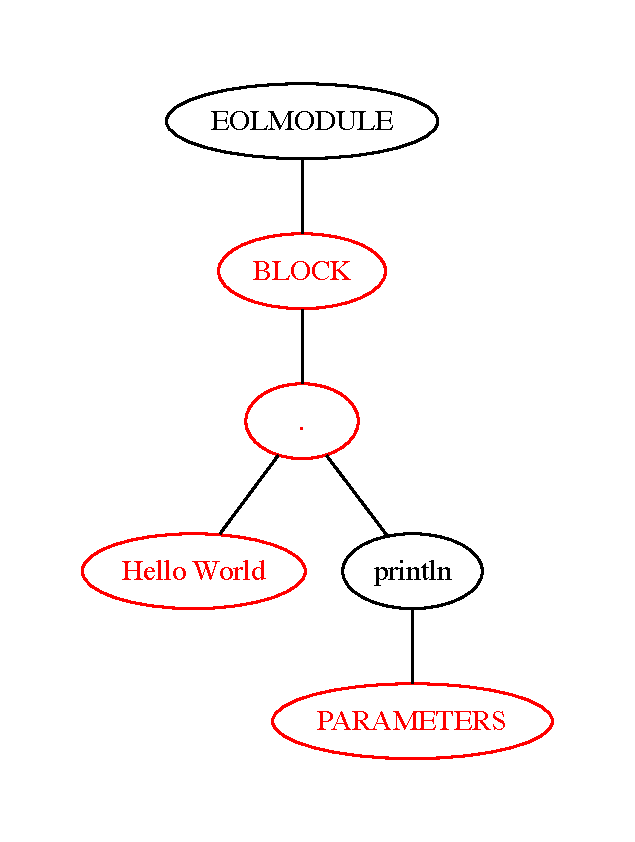
\includegraphics[scale=0.5]{figures/HelloWorldAST.pdf}
  \caption{The AST of the program in Figure \ref{lst:helloWorldEOL}}
  \label{fig:helloWorldAST}
\end{minipage}
\end{figure}

One approach for determining how many statements were executed would be to keep a list of visited AST vertices, and then count the total number of vertices in the AST. There is however a problem with this approach: Consider the very simple code in Figure \ref{lst:helloWorldEOL}, and the AST that is generated for the simple program as shown in Figure \ref{fig:helloWorldAST}. With that simple program, there is only 1 line that is going to be executed because there are no conditional statements that cause the program flow to change. However, the AST is comprised of 6 vertices. Testing shows that the execution listener's methods are only called on the red vertices. So while we know that the whole program has been executed, this naive approach will report only 4 out of 6 vertices have been executed.

Another approach that could be considered is to record which lines of the input file have been executed. This can be done because the AST class has a method called \verb+getLine()+ which as you would expect returns the line on which that statement comes from. So all of the red highlighted edges in Figure \ref{fig:helloWorldAST} return line 1 when \verb|getLine()| is called. So initial analysis would suggest that 1 out of 1 lines has been covered in the simple program in Figure \ref{lst:helloWorldEOL}, which is accurate. The problem with this was discussed in the literature review, and that is that it relies on two statements not being placed on the same line. The code in Figure \ref{lst:ifElseEOL} and its accompanying AST in Figure \ref{fig:ifElseAST} demonstrate this problem. Line coverage correctly is 100\%, because 1 out of 1 lines have been executed. However, not all of that 1 line has been executed, and so this is not an accurate reflection of the coverage. With the AST, 7 out of 14 vertices have been executed, which is a lot more accurate than the line coverage.

\begin{figure}
\centering
\begin{minipage}{.5\textwidth}
  \centering
  \lstinputlisting{code/ifElse.eol}
  \caption{An if/else EOL program}
  \label{lst:ifElseEOL}
\end{minipage}%
\begin{minipage}{.5\textwidth}
  \centering
  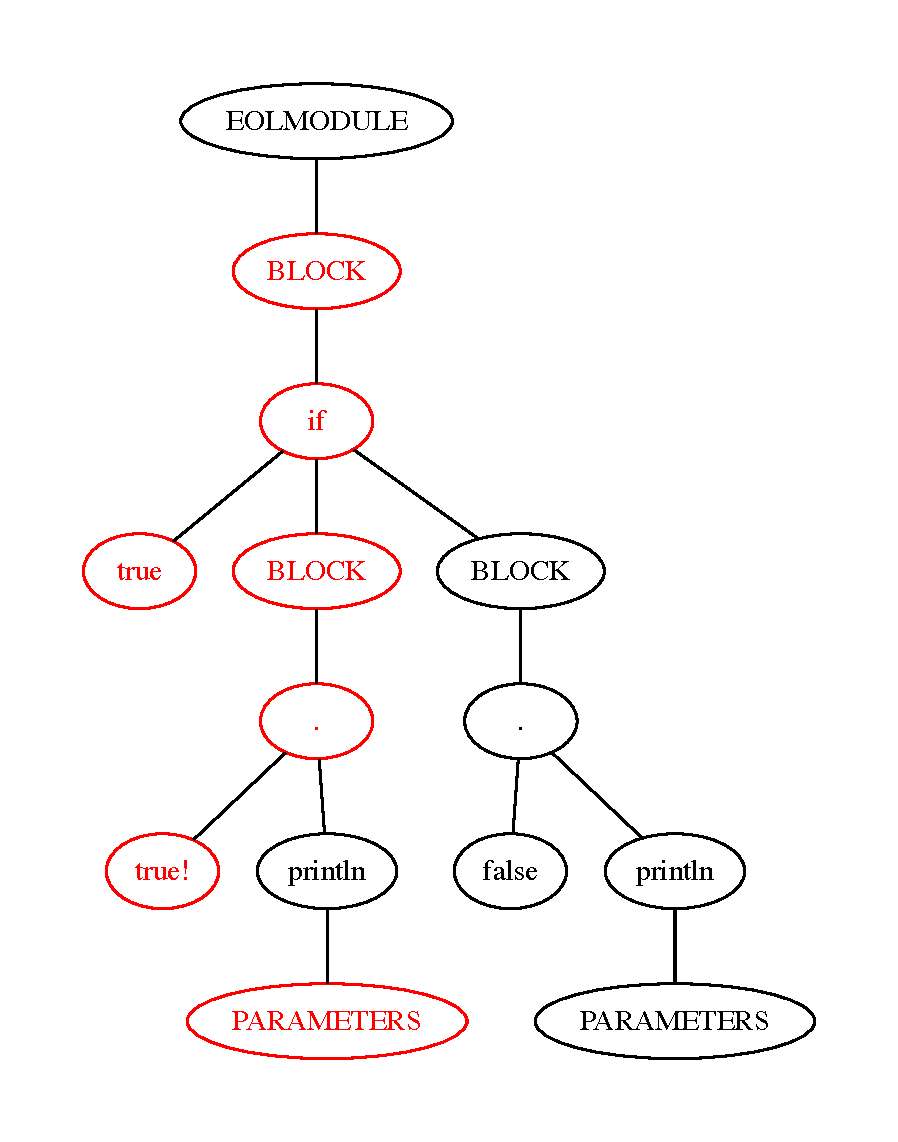
\includegraphics[scale=0.5]{figures/ifElseAST.pdf}
  \caption{The AST of the program in Figure \ref{lst:ifElseEOL}}
  \label{fig:ifElseAST}
\end{minipage}
\end{figure}

Thankfully another option is available. The AST class has a method called \verb|isImaginary()| which returns true when the current vertex is `imaginary'. While no documentation is available, it appears that vertices that can be directly mapped back to some text from the input file are not imaginary, and those that cannot be mapped back to some text are not. Figure \ref{fig:ifElseASTreal} shows the AST again, but this time with imaginary vertices left white, while non-imaginary vertices are filled in yellow. Quickly it becomes apparent that the definition of the method \verb+isImaginary()+ is not perfect as the vertex labelled EOLMODULE is coloured in yellow, despite not being directly mappable to a single statement in the input code. 

\begin{figure}
	\centering
	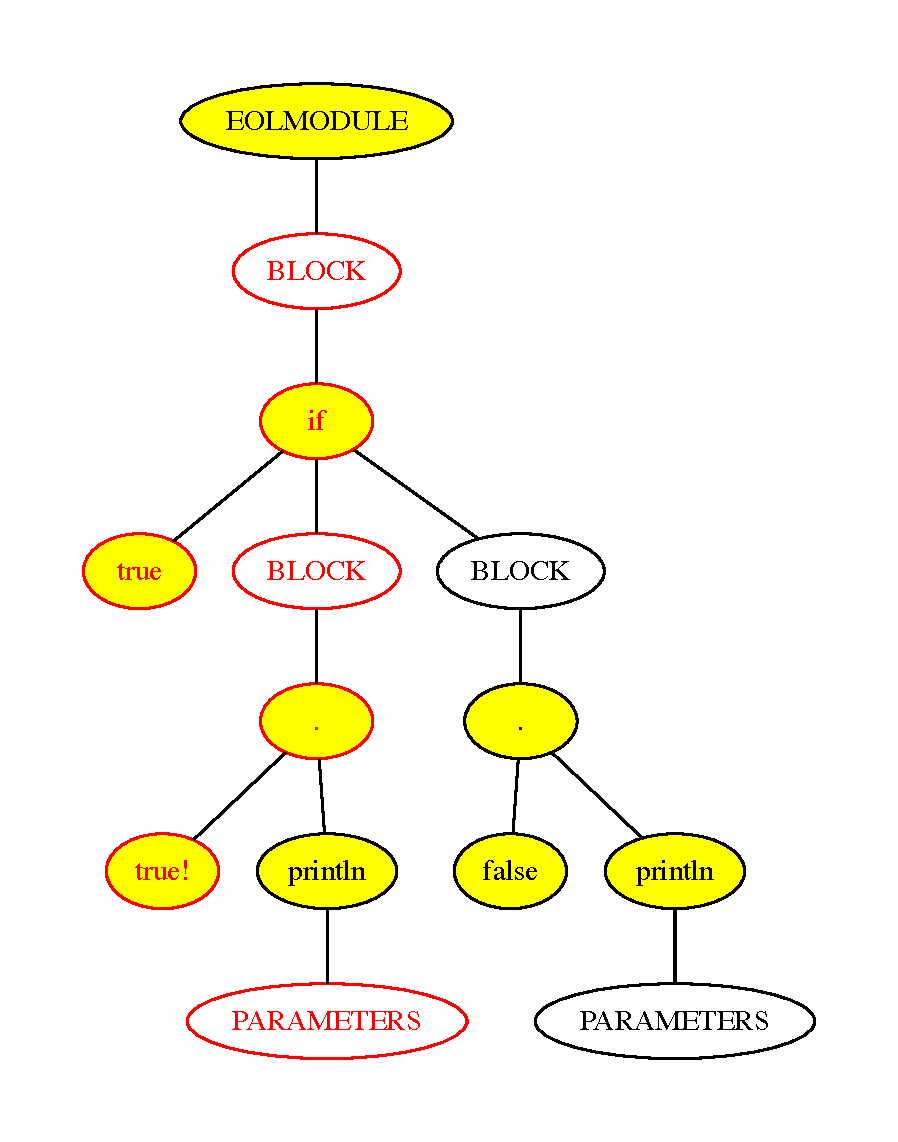
\includegraphics[scale=0.5]{figures/ifElseRealAST.pdf}
	\caption{The AST with yellow vertices being `real', and white vertices being `imaginary'}
	\label{fig:ifElseASTreal}
\end{figure}

\section{Design and Implementation}

When the EOL executor calls the execution listener's pre or post execute methods, there needs to be a way to store a reference to the AST that is passed into either of the methods.

An obvious way of doing this would be to have a list of references to the AST. When one of the pre or post-execute methods is fired, a check would be performed on the list to see if a reference to that particular AST vertex was already stored, and if not, it would be added to the list.

Once the program has completed execution, in order to satisfy requirements F-03 and F-04, an analysis must then be performed to determine which vertices have been executed, and which have not. To do this, each vertex in the AST must be checked against the list of visited vertices. The AST can either be traversed by a depth or breadth-first algorithm. I have chosen to use a depth-first algorithm purely because it is easier to implement, and uses less storage space than the breadth-first (as no queue has to be stored).

At each recursion in the depth-first traversal, the list of visited vertices must be checked against the current vertex. This is therefore a O($n^2$) algorithm, which is not ideal as any sizeable programme can quickly slow down, which goes against requirement NF-01. 

A way around this problem then is to use a hashmap to store the visited vertices. When either the pre or post-execute methods of the execution listener are fired, the hashmap would use the AST instance as the key, and the value would be a boolean. To insert to the hashmap, the values \verb|<ast, true>| would be passed in (where \verb|ast| is the AST instance). Later during analysis, a simple call of the Java HashMap method \verb|containsKey| would suffice, as it would return true if the AST instance has been inserted into the hashmap, or false otherwise. The use of a boolean as the value is arbitrary and in fact any value would suffice. 

This approach better fits the requirement NF-02, although NF-01 could potentially still not be met. If the default hashing function is poor and causes many collisions then the performance could degrade to a similar level of the previously described approach using a list of references. A solution could be to implement a better hashing function, but it seems like a lot of effort for what may not even be a problem.

Both of the above solutions work around the Epsilon source code by storing information in new objects. However this is not actually a requirement - it is perfectly acceptable to modify the Epsilon code as long as it is justifiable. The most simple solution then is to modify the AST class so that it contains a boolean that stores whether or not that particular vertex has been executed. When initialised of course this boolean will be set to false, but when the post-execute function in the execution listener is called and it is passed an AST as a parameter, we can just change the value of the executed boolean within the AST. This has the advantage of meaning that recording that a vertex has been visited is guaranteed to be a O(1) operation (unlike the hashmap or list based solutions). Better still, when the analysis is performed after execution has completed, the lookup time to determine whether a vertex has been executed is also guaranteed to be O(1). Again this is unlike the hashmap or linked list based solutions, which were worst case O(n) lookup time.

With the core algorithms decided on, the structure of the actual code has yet to be decided upon, as well as the output from the code. There of course needs to be a class that implements the \verb|IExecutionListener| interface. As the AST is directly being modified, then there is no need to transfer any data out of the execution listener (the AST will be available through another module). There therefore needs to be a class that takes the AST as input, and produces output of some sort. So to summarise, there will be two classes implemented. One called \verb|StatementCoverageListener| that implements the execution listener interface, and another called \verb|StatementCoverageAnalyser| that analyses and outputs some information.

The format of the output must satisfy requirements F-03 and F-04. 
